%!TEX root = ../these.tex

\section{
  Визуализация геометрической информации
}
\label{sec:json.view}

На разных этапах
как научных исследований,
так и технологической подготовки производства,
возникает потребность визуализации разнообразной
геометрической информации,
такой как геометрия деталей
и ограничивающих их контуров,
положение допустимых точек врезки
и выключения инструмента,
маршруты,
получаемые в ходе
решения различных классов задач резки,
а также маршруты движения резака,
получаемые после обработки постпроцессором
и т.п.

Традиционным подходом к визуализации является
разработка специализированных графических утилит
либо отдельных графических представлений
в рамках больших программных систем.
Зачастую этот подход является оправданным,
но у него есть и свои недостатки ---
прежде всего усложнение процесса разработки
и тестирования программного обеспечения.
Кроме того,
полученные таким образом визуализации
могут использоваться,
например, для научных публикаций,
только посредством создания растровых копий экранов,
или же требуется разработка отдельной функциональности
для экспорта визуализации в файл некоторого формата.

Альтернативный подход,
зачастую оказывающийся
\textit{гораздо}
легче в разработке,
заключается в том,
чтобы визуализация производилась
путём экспорта в некоторый графический формат,
который уже может широко использоваться как
для распространения,
так и для собственно просмотра при помощи
стандартных утилит.
Стандартом де-факто в наше время
для этой цели является формат
SVG~\cite{bi:SVG},
а для его оперативного отображения
может использоваться любой современный браузер,
впрочем как и множество готовых библиотек
для встраивания в разрабатываемое программное обеспечение.
Важным достоинством такого подхода
является его кросс-платформенность,
то есть возможность использовать его
на большинстве платформ и операционных систем.

В данной диссертационной работе
как раз повсеместно и использовался формат SVG
при намеренном отказе от разработки
собственных программ визуализации.
Например,
в Листинге~\ref{lst:json-svg}
приводится простейший SVG-файл,
сгенерированный для раскройной карты,
представленной на Листинге~\ref{lst:json-dbs}.

\lstinputlisting[
  language=XML,
  basicstyle=\footnotesize,
  showstringspaces=false,
  numbers=left,
  label={lst:json-svg},
  captionpos=b,
  caption=SVG-файл для визуализации раскроя из Листинга~\ref{lst:json-dbs}
  ]
  {media/nesting.svg}

Можно заметить,
что команды SVG
практически идеально соответствуют
элементам геометрической информации.
Фактически,
SVG может использоваться даже
как альтернативный вариант
хранения и обмена графической информацией
(вместо DXF, DBS, JSON\dots),
хотя в данной работе этого не происходило,
утилиты раздела~\ref{sec:json-dbs.js}
только экспортируют в SVG
без возможности обратного преобразования.

\subsection{Настройка параметров визуализации}

Переход к широкому использованию SVG
позволяет также использовать зрелые современные технологии
каскадных таблиц стилей
(Cascading Style Sheets, CSS)
для управления внешним видом визуализации
(включая цвета, заливки и штриховки и анимацию)
и язык JavaScript
для добавления к визуализации
элементов интерактивности.
Один из вариантов оформления
SVG-файла из Листинга~\ref{lst:json-svg}
приведён на рис.~\ref{fig:json-nesting}.
Пользовательский интерфейс
(масштабирование и прокрутка)
обеспечивается при помощи подключения
библиотеки с открытым кодом
svg-pan-zoom~\cite{bi:svg-pan-zoom}.

\begin{figure}
  \centering
  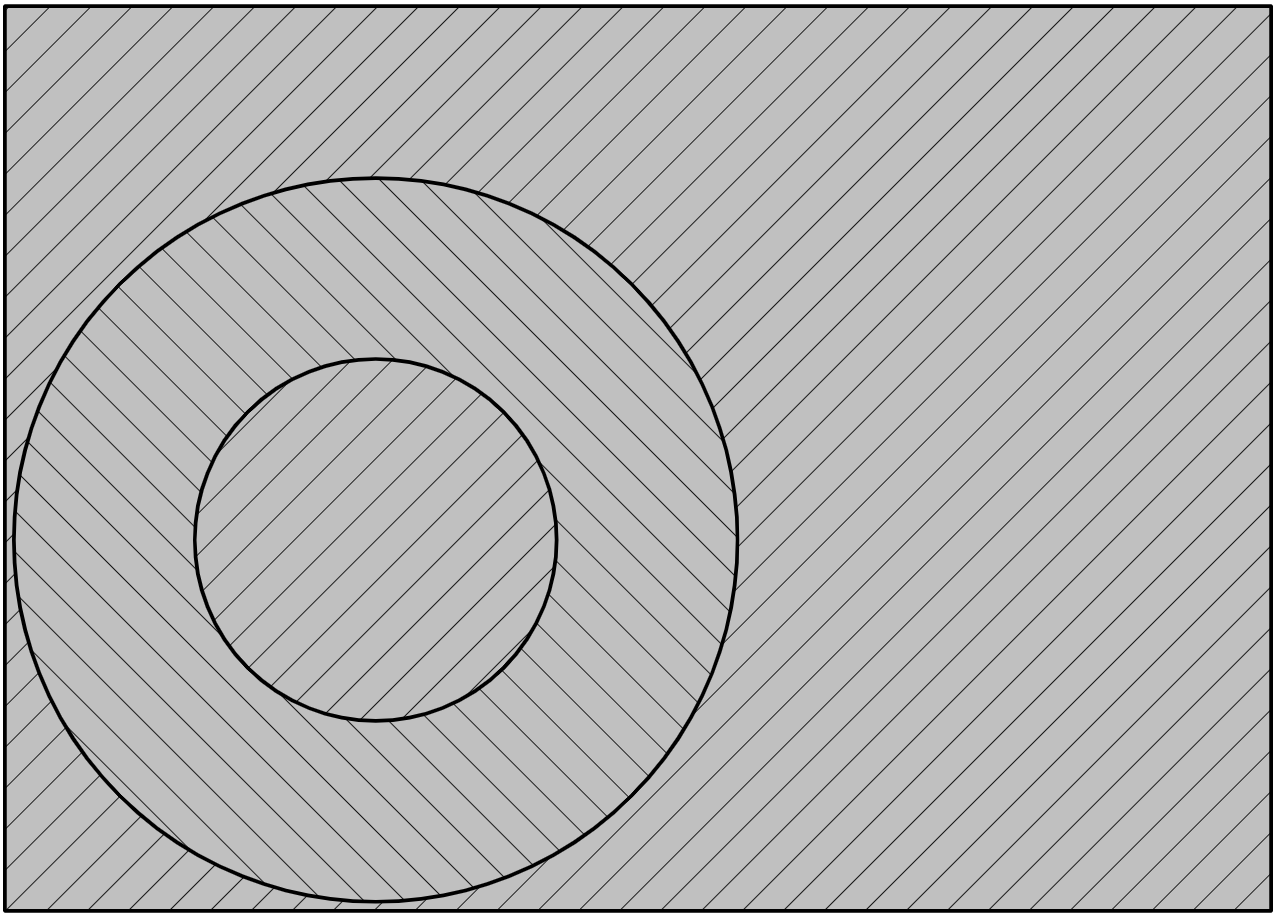
\includegraphics[width=0.5\textwidth]{nesting.png}
  \caption{Визуализация раскроя из Листинга~\ref{lst:json-dbs}}
  \label{fig:json-nesting}
\end{figure}

В ходе диссертационной работы
была разработан пакет утилит
\cite{bi:dbs2json},
обеспечивающих конвертацию между
различными форматами файлов
(включая DBS, JSON, YAML, DXF и SVG для визуализации).
Для визуализации решения задачи PCGTSP
(на основе комбинации информации,
полученной из нескольких источников),
была разработана специализированная утилита
\cite{bi:j2pcgtsp},
первоначально в форме утилиты командной строки
но позднее преобразованная
для удобства использования в
Single Page Application
(SPA).
Пример созданного ею изображения
приведён на рис.~\ref{fig:pcgtsp.svg},
стр.~\pageref{fig:pcgtsp.svg}.
